\documentclass{article}
\usepackage{graphicx}
\usepackage{amsmath}
\usepackage{pgfplots}
\usepackage{physics}
\usepackage{cancel}
\usepackage{enumitem}
\usepackage{txfonts}
\usepackage[normalem]{ulem}

\pgfplotsset{compat=1.18}

\pgfplotsset{compat=1.18}

\usepackage[a4paper, top=1cm, bottom=2cm, left=2cm, right=2cm, includehead, includefoot]{geometry}

\begin{document}

\noindent
Physics 4B - Electromagnetism \hfill Prof. Alfred Cauthen
\noindent\rule{\textwidth}{0.4pt}

\begin{center}
    \textbf{\LARGE Homework 1} \\
    \vspace{12pt}
    \large Aaron W. Tarajos \\
    \textit{\today}
\end{center}

\noindent\rule{\textwidth}{0.4pt}

\section*{21-3 Question 2}
Figure 21-12 shows three pairs of identical spheres that are to be touched together and then separated.
The initial charges on them are indicated.
Rank the pairs according to (a) the magnitude of the charge transferred during touching and (b) the charge left on the positively charged sphere, greatest first.

\begin{figure}[ht]
    \centering
    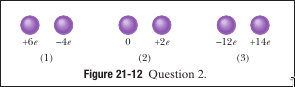
\includegraphics[scale=0.75]{image.png}
\end{figure}

\subsection*{Solution}
\textbf{Part a:} The first pair transfers $4e$, the second pair transfers $0e$ of chrage, and the third pair transfers $12e$ of charge.

\[
    \boxed{\text{pair 3}  > \text{pair 1} > \text{pair 2}}
\]
\textbf{Part b:} The positively charged sphere is left with $2e$ in all three transfers.

\section*{21-3 Question 8}
Figure 21-17 shows four arrangements of charged particles.
Rank the arrangements according to the magnitude of the net electrostatic force on the particle with charge +Q, greatest first.

\begin{figure}[ht]
    \centering
    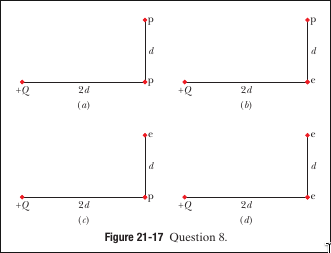
\includegraphics[scale=0.75]{image-2.png}
\end{figure}

\subsection*{Solution}
The forces magnitude in $(a)$ and $(d)$ are the same because the configuration of the system is the same just with the opposite charge which changes the direction of the force not the magnitude.
The same can be said for the relationship between $(b)$ and $(c)$, although their magnitude is less than the other configuration because the difference in charge of the particles acting on $Q$ create forces of the opposite sign in one direction which reduces the magnitude of the total force.
Therefore we have;

\[
    \boxed{a = d > b = c}
\]

\section*{21-3 Question 10}
In Fig.21-19, a central particle of charge $-2q$ is surrounded by a square array of charged particles, separated by either distance $d$ or $d/2$ along the perimeter of the square.
What are the magnitude and direction of the net electrostatic force on the central particle due to the other particles?

\begin{figure}[ht]
    \centering
    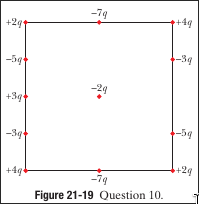
\includegraphics[scale=0.75]{image-3.png}
\end{figure}

\subsection*{Solution}
Notice that every single charge has a charge on of equal magnitude exactly opposite to it in the system with exception of the $+3q$ charge to the left of the central particle.
Therefore the net force in every other direction will sum to zero with the exception of that one where we have;

\[
	F_e = k \frac{|3||-2|}{d^2/2^2} = \boxed{k \frac{24}{d^2}\ \text{N} \quad \text{to the left}}
\]

\section*{21-3 Problem 10}
In Fig. 21-25, four particles form a square. The charges are $q1 = q4 = Q$ and $q2 = q3 = q$.
(a) What is $Q/q$ if the net electrostatic force on particles 1 and 4 is zero?
(b) Is there any value of q that makes the net electrostatic force on each of the four particles zero? Explain.

\begin{figure}[ht]
    \centering
    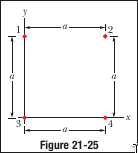
\includegraphics[scale=0.75]{image-4.png}
\end{figure}

\subsection*{Solution}
\textbf{Part a:} From the symmetry we just need to find the $Q/q$ such that
\[
    F_{14,y} + F_{13} = 0
\]
which we can find by

\begin{align*}
    F_{14,y} &= k \frac{Q^2}{\left(\sqrt{2a^2}\right)^2} \sin\left(\frac{\pi}{4}\right)\\
    &= k \frac{Q^2}{2a^2} \cdot \frac{1}{\sqrt{2}}
\end{align*}
and

\begin{align*}
    F_{13} &= k \frac{Qq}{a^2}
\end{align*}
then

\begin{align*}
    k \frac{Q^2}{2a^2\sqrt{2}} + k \frac{Qq}{a^2} &= 0 \\
    k \frac{Q^2}{2a^2\sqrt{2}} &= - k \frac{Qq}{a^2} \\
    \frac{Q^2}{2\sqrt{2}} &= - Qq \\
    \frac{Q}{q} &= \boxed{- 2 \sqrt{2}}
\end{align*}
\textbf{Part b:} No, there is no value of $q$ that would result in each of the net forces being zero because of the mirror symmetry of the configuration.
Meaning that $q/Q = -2\sqrt{2}$ if the net force on particle 3 is zero and it cannot be simultaneosly true that $q/Q = -2\sqrt{2} \wedge Q/q = -2\sqrt{2}$.

\section*{21-3 Problem 11}
In Fig. 21-25, the particles have charges $q_1 = -q_2 = 100$ nC and $q_3 = -q_4 = 200$ nC, and distance $a = 5.0$ cm.
What are the (a) $x$ and (b) $y$ components of the net electrostatic force on particle 3?

\subsection*{Solution}
\textbf{Part a:} We have two forces acting on particle 3 in the $x$ direction, one being the force from particle 4 and the other being the $x$ component of particle 2.
Both forces are attractive so we have.

\begin{align*}
    F_{3, x} &= k \frac{|q_3||q_4|}{a^2} + k \frac{|q_3||q_2|}{2a^2} \cdot \frac{1}{\sqrt{2}} \\
    &= k \left( \frac{|q_3||q_4|}{a^2} + \frac{|q_3||q_2|}{2a^2\sqrt{2}} \right) \\
    &= 8.99 \times 10^9 \cdot \text{N} \frac{\text{m}^2}{\text{C}^2} \left( \frac{|200||-200|}{5.0^2} \frac{\text{n$^2$C}^2}{\text{m}^2} + \frac{|200||-100|}{2(5.0^2)} \frac{1}{\sqrt{2}} \frac{\text{n$^2$C}^2}{\text{m}^2} \right) \\
    &= 8.99 \times 10^9 \cdot \text{N} \frac{\text{m}^2}{\text{C}^2} \left( \frac{40000}{25.0} + \frac{20000}{50.0 \sqrt{2}}  \right) \frac{\text{n$^2$C}^2}{\text{m}^2}\\
    &= \boxed{1.7 \times 10^{-5} \ \text{N}}
\end{align*}
\textbf{Part b:} Again we have two forces but now they are acting in opposite directions.
The $y$ component of the force from particle 2 on particle 3 is in the positive y direction and the force from particle 1 on particle 3 is in the negative y direction.
Therefore we have;

\begin{align*}
    F_{3, y} &= -k \frac{|q_3||q_1|}{a^2} + k \frac{|q_3||q_2|}{2a^2} \cdot \frac{1}{\sqrt{2}} \\
    &= k \left( -\frac{|q_3||q_1|}{a^2} + \frac{|q_3||q_2|}{2a^2\sqrt{2}} \right) \\
    &= 8.99 \times 10^9 \cdot \text{N} \frac{\text{m}^2}{\text{C}^2} \left( -\frac{|200||100|}{5.0^2} \frac{\text{n$^2$C}^2}{\text{m}^2} + \frac{|200||-100|}{2(5.0^2)} \frac{1}{\sqrt{2}} \frac{\text{n$^2$C}^2}{\text{m}^2} \right) \\
    &= 8.99 \times 10^9 \cdot \text{N} \frac{\text{m}^2}{\text{C}^2} \left( -\frac{20000}{25.0} + \frac{20000}{50.0 \sqrt{2}}  \right) \frac{\text{n$^2$C}^2}{\text{m}^2}\\
    &= \boxed{4.6 \times 10^{-6} \ \text{N}}
\end{align*}

\section*{21-3 Problem 23}
In Fig. 21-32, particles 1 and 2 of charge $q_1 = q_2 = +3.20 \times 10^{-19}$ C are on a $y$ axis at distance $d = 17.0$ cm from the origin.
Particle 3 of charge $q_3 = +6.40 \times 10^{-19}$ C is moved gradually along the $x$ axis from $x = 0$ to $x = +5.0$ m.
At what values of x will the magnitude of the electrostatic force on the third particle from the other two particles be
(a) minimum and
(b) maximum? What are
the
(c) minimum and
(d) maximum magnitudes?

\begin{figure}[ht]
    \centering
    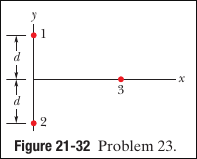
\includegraphics[scale=0.75]{image-5.png}
\end{figure}

\subsection*{Solution}
\textbf{Part a:} The vertical component of the force on 3 by 1 is the same but in the opposite direction of the force on 3 by 2. Therefore, the net vertical force is zero and so the only thing that matters is the horizontal component of the forces. That means the force will be at a minimum when the there is no horizontal force component which is at $x = 0$. \vspace{12pt} \\
\textbf{Part b:} We can write the horizontal force component as
\begin{align*}
	F_{31} &= k \frac{q_1q_3}{x^2 + d^2} \cdot \vu r \\
	&= k \frac{q_1q_3}{x^2 + d^2} \cdot \frac{\va r}{\sqrt{x^2 + d^2}} \\
	&= k \frac{q_1q_3}{x^2 + d^2} \cdot \frac{x\ \vu i + d\ \vu j}{\sqrt{x^2 + d^2}} \\
	&= \left( k \frac{q_1q_3}{x^2 + d^2} \cdot \frac{x}{\sqrt{x^2 + d^2}} \right)\ \vu i
\end{align*}
and again because of the symmetry our horizontal force is just twice this. So we can find the extremal points this function;
\begin{align*}
	F_{31}^\prime &= k q_1 q_3 \frac{d}{dx}\left[\frac{x}{\sqrt{x^2 + d^2}^3}\right] \\
		      &= k q_1 q_3 \frac{\left(x^2 + d^2\right)^{3/2} - 3x^2\sqrt{x^2 + d^2}}{\left( x^2 + d^2 \right)^{6/2}} \\
		      &= k q_1 q_3 \frac{\left(x^2 + d^2\right) - 3x^2}{\left( x^2 + d^2 \right)^{5/2}}
\end{align*}
which we now set equal to zero and solve for $x$;
\begin{align*}
	k q_1 q_3 \frac{\left(x^2 + d^2\right) - 3x^2}{\left( x^2 + d^2 \right)^{5/2}} &= 0 \\
	x^2 + d^2 - 3x^2 &= 0 \\
	2x^2 &= d^2 \\
	x &= \sqrt{\frac{d^2}{2}} \\
	x &= \sqrt{\frac{0.17^2}{2}} \\
	x &= \boxed{0.12\ \text{m}}
\end{align*}
\textbf{Part c:} The mimum magnitude is 0 N, because we can see that our force equation in (b) is zero when $x=0$. \vspace{12pt} \\
\textbf{Part d:} We plugin our result for $x$ from part (b) into the equation for the force;
\begin{align*}
	F_\text{net} &= 2 \left( k \frac{q_1q_3}{x^2 + d^2} \cdot \frac{x}{\sqrt{x^2 + d^2}} \right) \\
	&= 2 \left( 8.988 \times 10^9 \frac{3.20 \times 10^{-19} \cdot 6.40 \times 10^{-19}}{0.12^2 + 0.17^2} \cdot \frac{0.12}{\sqrt{0.12^2 + 0.17^2}} \right) \\
	&= \boxed{4.903\times 10^{-26}\ \text{N}}
\end{align*}

\section*{21-3 Problem 31}
Earth’s atmosphere is constantly bombarded by cosmic ray protons that originate somewhere in space.
If the protons all passed through the atmosphere, each square meter of Earth’s surface would intercept protons at the average rate of 1500 protons per second.
What would be the electric current intercepted by the total surface area of the planet?
\subsection*{Solution}
The surface of the earth is $5.1 \times 10^{11}$ m$^2$, so we have a total of
\[
	1500 \cdot 5.1 \times 10^{14} = 7.65 \times 10^{17}\ \text{protons}/\text{s}
\]
protons per second and then the current is given by charge per second and each proton has a charge of $1.602 \times 10^{-19}$ C. So we have;
\[
	7.650 \time 10^{17} \cdot 1.602 \times 10^{-19} = \boxed{0.12\ \text{A}}
\]

\section*{21-3 Problem 36}
Electrons and positrons are produced by the nuclear transformations of protons and neutrons known as beta decay.
(a) If a proton transforms into a neutron, is an electron or a positron produced?
(b) If a ­ neutron transforms into a proton, is an electron or a positron produced?

\subsection*{Solution}
\textbf{Part a:} A positron is produced because the proton needs lose positive charge to become neutral. \vspace{12pt}\\
\textbf{Part b:} A electron is produced because the neutron needs to lose negative charge to become positively charged.

\end{document}
